\documentclass{beamer}

%% Load Latex packages
\usepackage{amssymb}
\usepackage{color}
\usepackage{float}
\usepackage[T1]{fontenc}
\usepackage{graphicx}
\usepackage{hyperref}
\usepackage[utf8]{inputenc}
\usepackage{lmodern}
\usepackage{makecell}
\usepackage[authoryear, round]{natbib}
\usepackage{ragged2e}
\usepackage{tikz} %% For drawing arrows
\usepackage{wrapfig}
\usepackage{xmpincl}
\usepackage{xspace}

%% Colors
%% ------
% Color panel used throughout the poster
\definecolor{lgray}{rgb}{0.9179688,0.9179688,0.9179688} % #ebebeb
\definecolor{dgray}{rgb}{0.796875,0.796875,0.796875} % #cccccc
\definecolor{vdgray}{rgb}{0.3984375,0.3984375,0.3984375} % #666666
\definecolor{coral}{rgb}{0.9960938,0.4960938,0.3125000} % #ff7f50
\definecolor{blue}{rgb}{0.4218750,0.6484375,0.8007812} % #6ca6cd
\definecolor{green}{rgb}{0.6992188,0.7265625,0.5078125} % #b3ba82
\definecolor{yellow}{rgb}{0.9570312,0.8671875,0.6992188} % #f5deb3


%% Coding fonts
%% ------------
%% Font for R chunks
\usepackage{listings}
\lstset{
  language=R,
  basicstyle=\tiny\ttfamily\color{vdgray}, % the size of the fonts that are used for the code
  numbers=left,                   % where to put the line-numbers
  numberstyle=\tiny\color{gray},  % the style that is used for the line-numbers
  stepnumber=1,                   % the step between two line-numbers.
  numbersep=0.1cm,                % how far the line-numbers are from the code
  backgroundcolor=\color{lgray},  % choose the background color. You must add \usepackage{color}
  deletekeywords={stat, model, matrix},
  keywordstyle=\color{blue},      % keyword style
  stringstyle=\color{green},      % string literal style
  xleftmargin=0.5cm,
}

%% Adapt template format 
%% ------------
%% headline
\setbeamercolor{section in head/foot}{bg=lgray, fg=black}
%% frametitle 
\setbeamerfont{frametitle}{series=\bfseries}
\setbeamercolor{frametitle}{bg=lgray, fg=black}
%% table of content
\setbeamercolor{section in toc}{fg=black}
\setbeamerfont{section in toc}{size=\large}
%% footer
\setbeamertemplate{footline}[text line]{
  \parbox{\linewidth}{
    \small
    \hfill
    \color{vdgray}{\insertframenumber}
    \hspace{-1cm}
    \vspace{0.3em}
  }
}
%% Remove the navigati
\beamertemplatenavigationsymbolsempty

%% Custom functions
%% ------------
%% Inline code highlight
\newcommand{\hcode}[2][lgray]{{\ttfamily\color{vdgray}\colorbox{#1}{#2}}}

%% Presentation metadata
%% ------------
\title{A standardized computational framework for the analysis of mass 
spectrometry-based single-cell proteomics data}
\author[]{Christophe Vanderaa, Laurent Gatto}
\date{December 18, 2020}

\begin{document}

%% Apply the 'remember picture' style to all pictures that defines or uses
%% external nodes
\tikzstyle{every picture}+=[remember picture]

%% Title page
\begin{frame}[plain]
\titlepage
\centering

\includegraphics[width=0.15\linewidth]{figs/eurobioc2020.jpg}
\end{frame}

%% Single-cell technology
\begin{frame}[c]
  \frametitle{Single-cell technology}
  
  \textbf{Single-cell omics} generate measurements for one cell
  
  \vfill
  \begin{columns}
    \column{0.45\linewidth}
    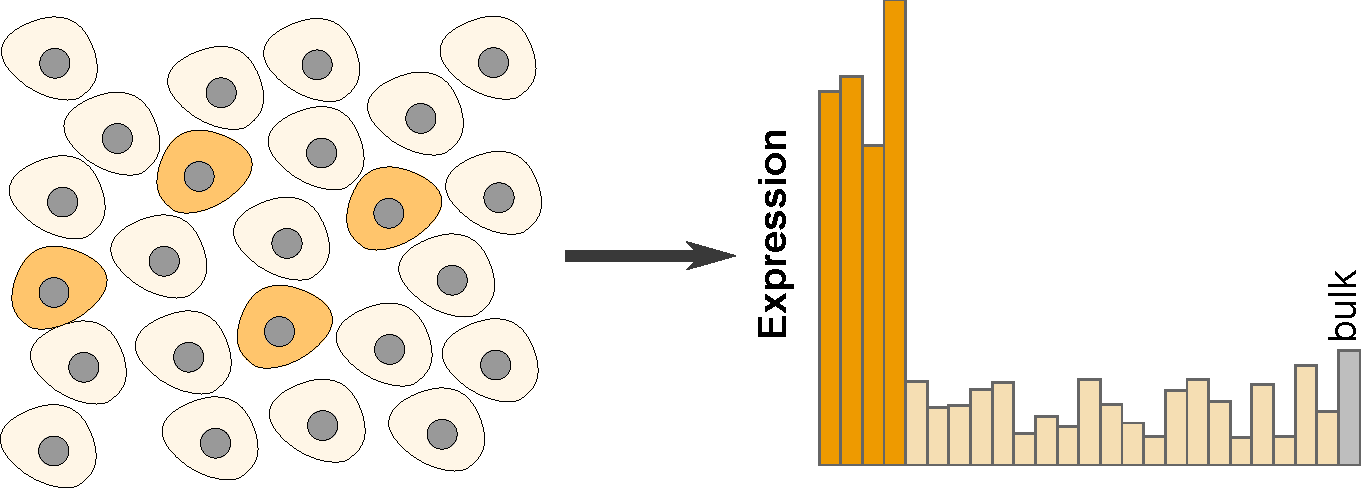
\includegraphics[width=\linewidth]{figs/bulk_issue1.pdf}
    \column{0.45\linewidth}
    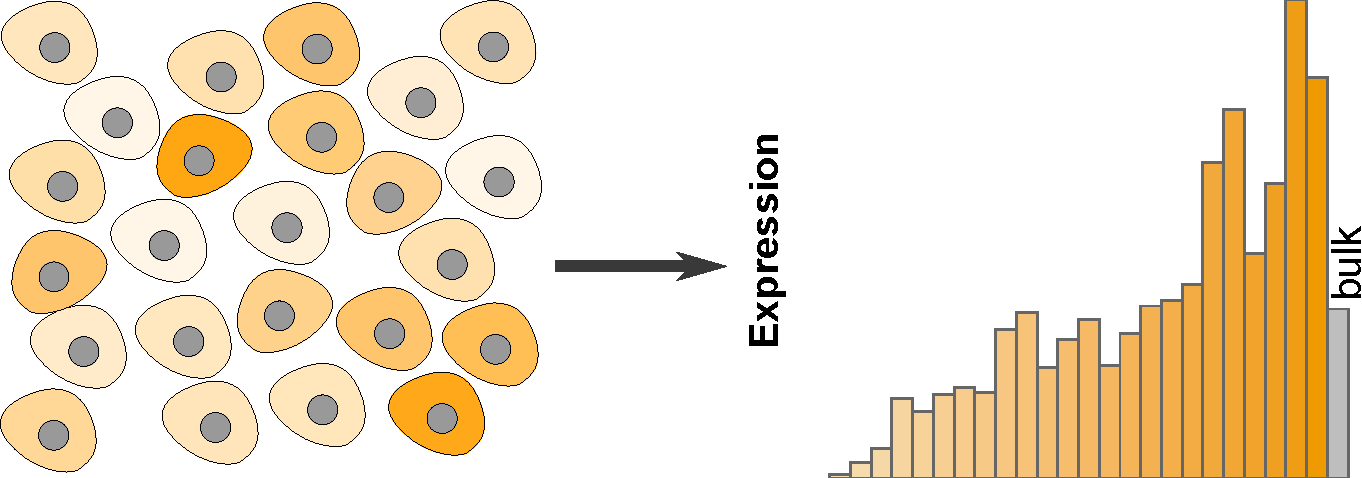
\includegraphics[width=\linewidth]{figs/bulk_issue2.pdf}
  \end{columns}
  
  \vfill
  scRNA-Seq is maturing very quickly with several standardized 
  pipelines, e.g. OSCA book (\cite{Amezquita2019-bf})
  
  \vfill
  \textbf{BUT} cellular fonction is driven by proteins
  
\end{frame}

%% Single-cell proteomics 
\begin{frame}[c]
  \frametitle{Single-cell proteomics }
  
  \begin{columns}
  
    \column{0.5\linewidth}
    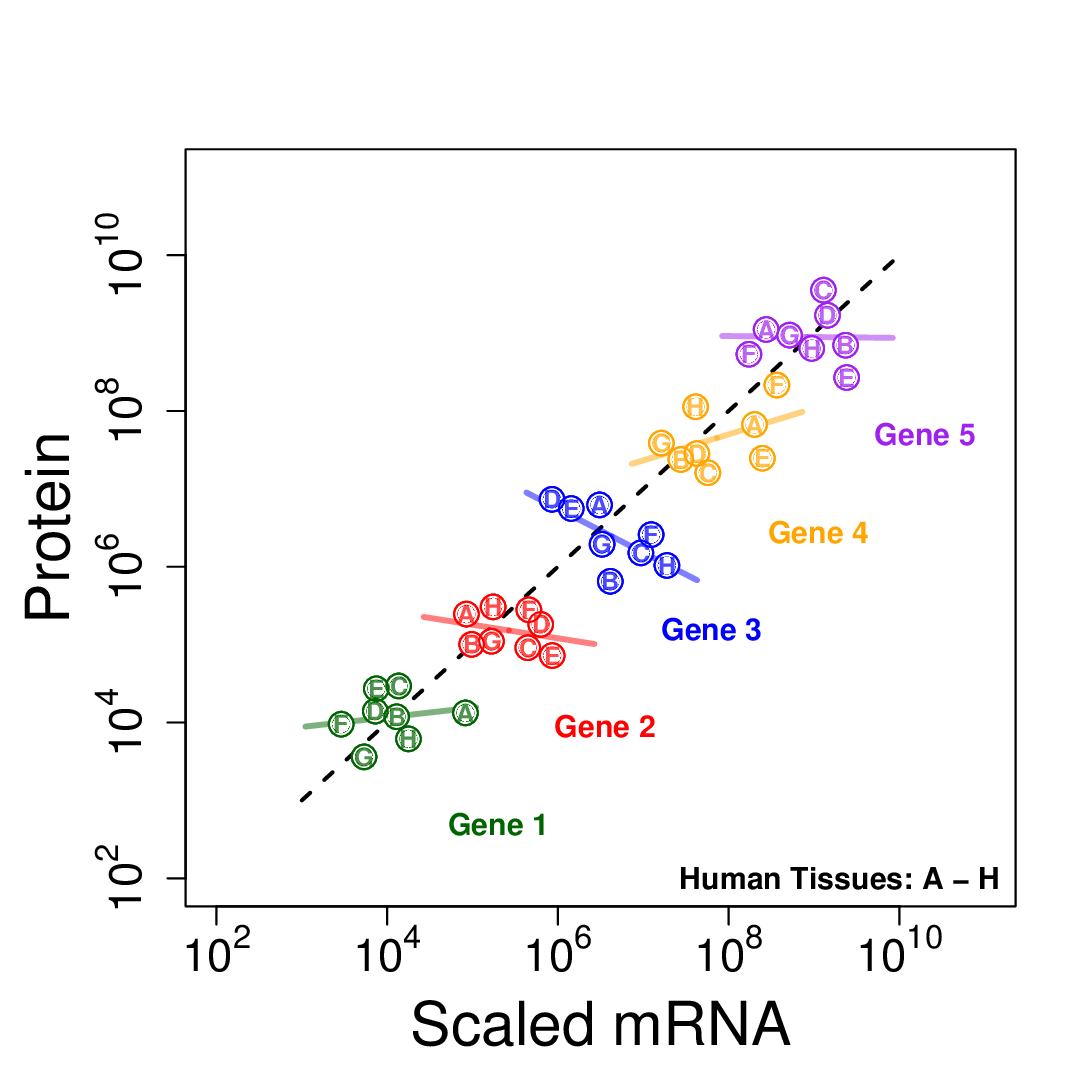
\includegraphics[width=\linewidth]{figs/simsons_paradox_in_gene_regulation.png}
    \footnotesize
    Source: \cite{Specht2018-hi}
    
    \pause
    \column{0.5\linewidth}
    \textbf{Flow cytometry or CITE-Seq}
    \begin{itemize}
      \item High throughput
      \item High sensitivity
    \end{itemize}
    \vspace{0.5cm}
    \textbf{BUT} antibody based:\\
    \begin{itemize}
      \item Targeted approach
      \item Specificity issues
    \end{itemize}
  
  \end{columns}
  
\end{frame}

%% MS-based single-cell proteomics
\begin{frame}[allowframebreaks, b]
  \frametitle{MS-based single-cell proteomics}
  
  \begin{center}
    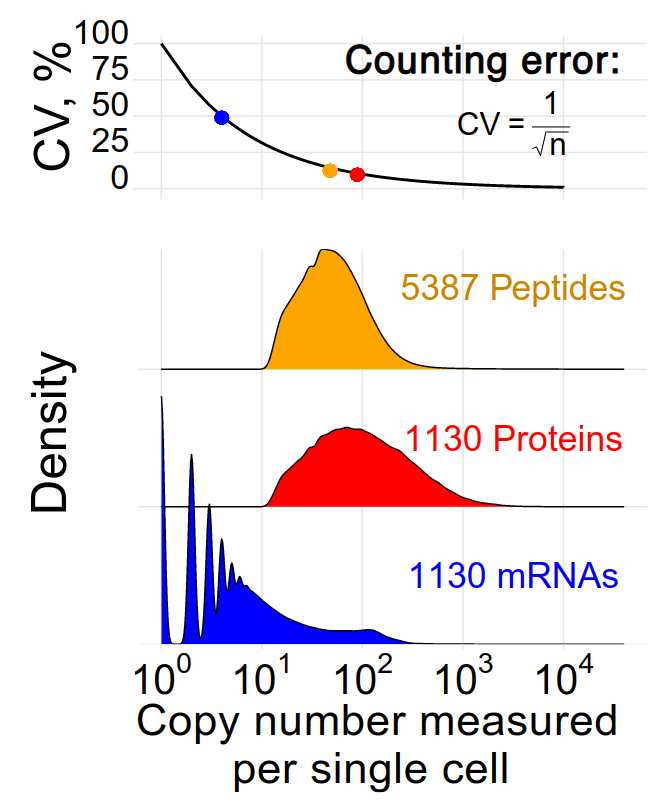
\includegraphics[width=0.5\linewidth]{figs/Counting_error.png}\\
    Source: \cite{Specht2020-jm}
  \end{center}
  
  \framebreak
  
  Recent milestone : SCoPE2 protocol {\footnotesize(\cite{Specht2020-jm})}
  \begin{itemize}
    \item $\sim$ 1500 single cells 
    \item $\sim$ 3000 quantified proteins
    \item $\sim$ 600 proteins expressed per cell
  \end{itemize}

  \vfill
  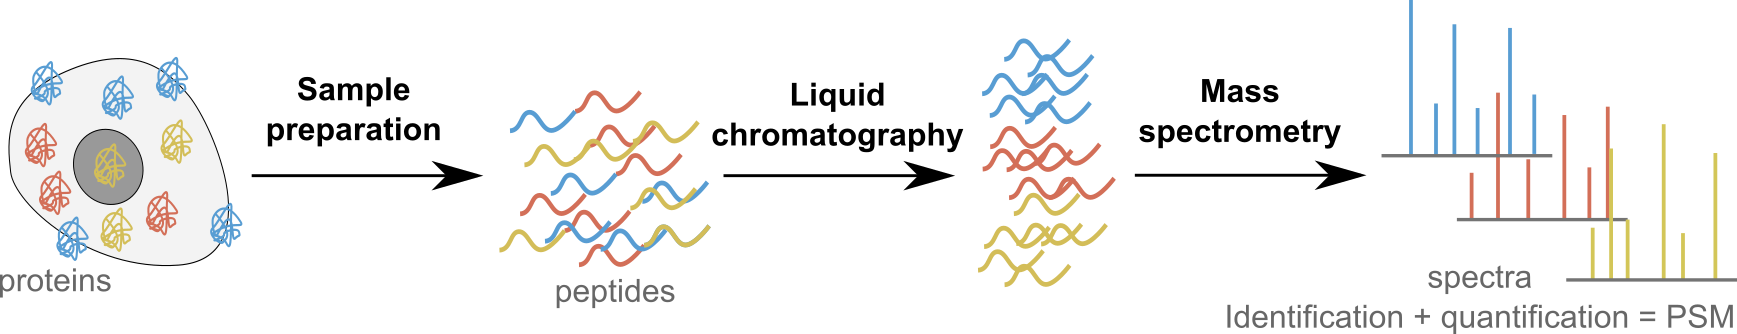
\includegraphics[width=\linewidth]{figs/MS-SCP.png}
  
  \vfill
  Between 1 (label-free) and 10 (TMT multiplexing) single cells per run
  \vfill
  
\end{frame}

%% Our contribution
\begin{frame}
  \frametitle{Our contribution}
  
  We offer a solution to the \textbf{lack of good computational tools}
  for handling SCP data.

  \vfill
  \begin{itemize}
    \item SCP data framework combines existing Bioconductor classes
    \item \hcode{scpdata} disseminates curated SCP data sets 
    for method development and benchmarking (soon on Bioconductor)
    \item \hcode{scp} implements functions to streamline the 
    analysis of SCP data (available on Bioconductor)
  \end{itemize}

\end{frame}

%% Data framework
\begin{frame}[allowframebreaks]
  \frametitle{Data framework}
  
  \vfill 
  \begin{columns}
    \column{0.5\linewidth}
    \centering
    \textbf{Single-cell}
    \column{0.5\linewidth}
    \centering
    \textbf{Proteomics}
  \end{columns}
  \vfill
  \begin{columns}
    \column{0.5\linewidth}
    \centering
    
\includegraphics[width=0.3\linewidth]{figs/sticker_SCE.png}
    \column{0.5\linewidth}
    \centering
    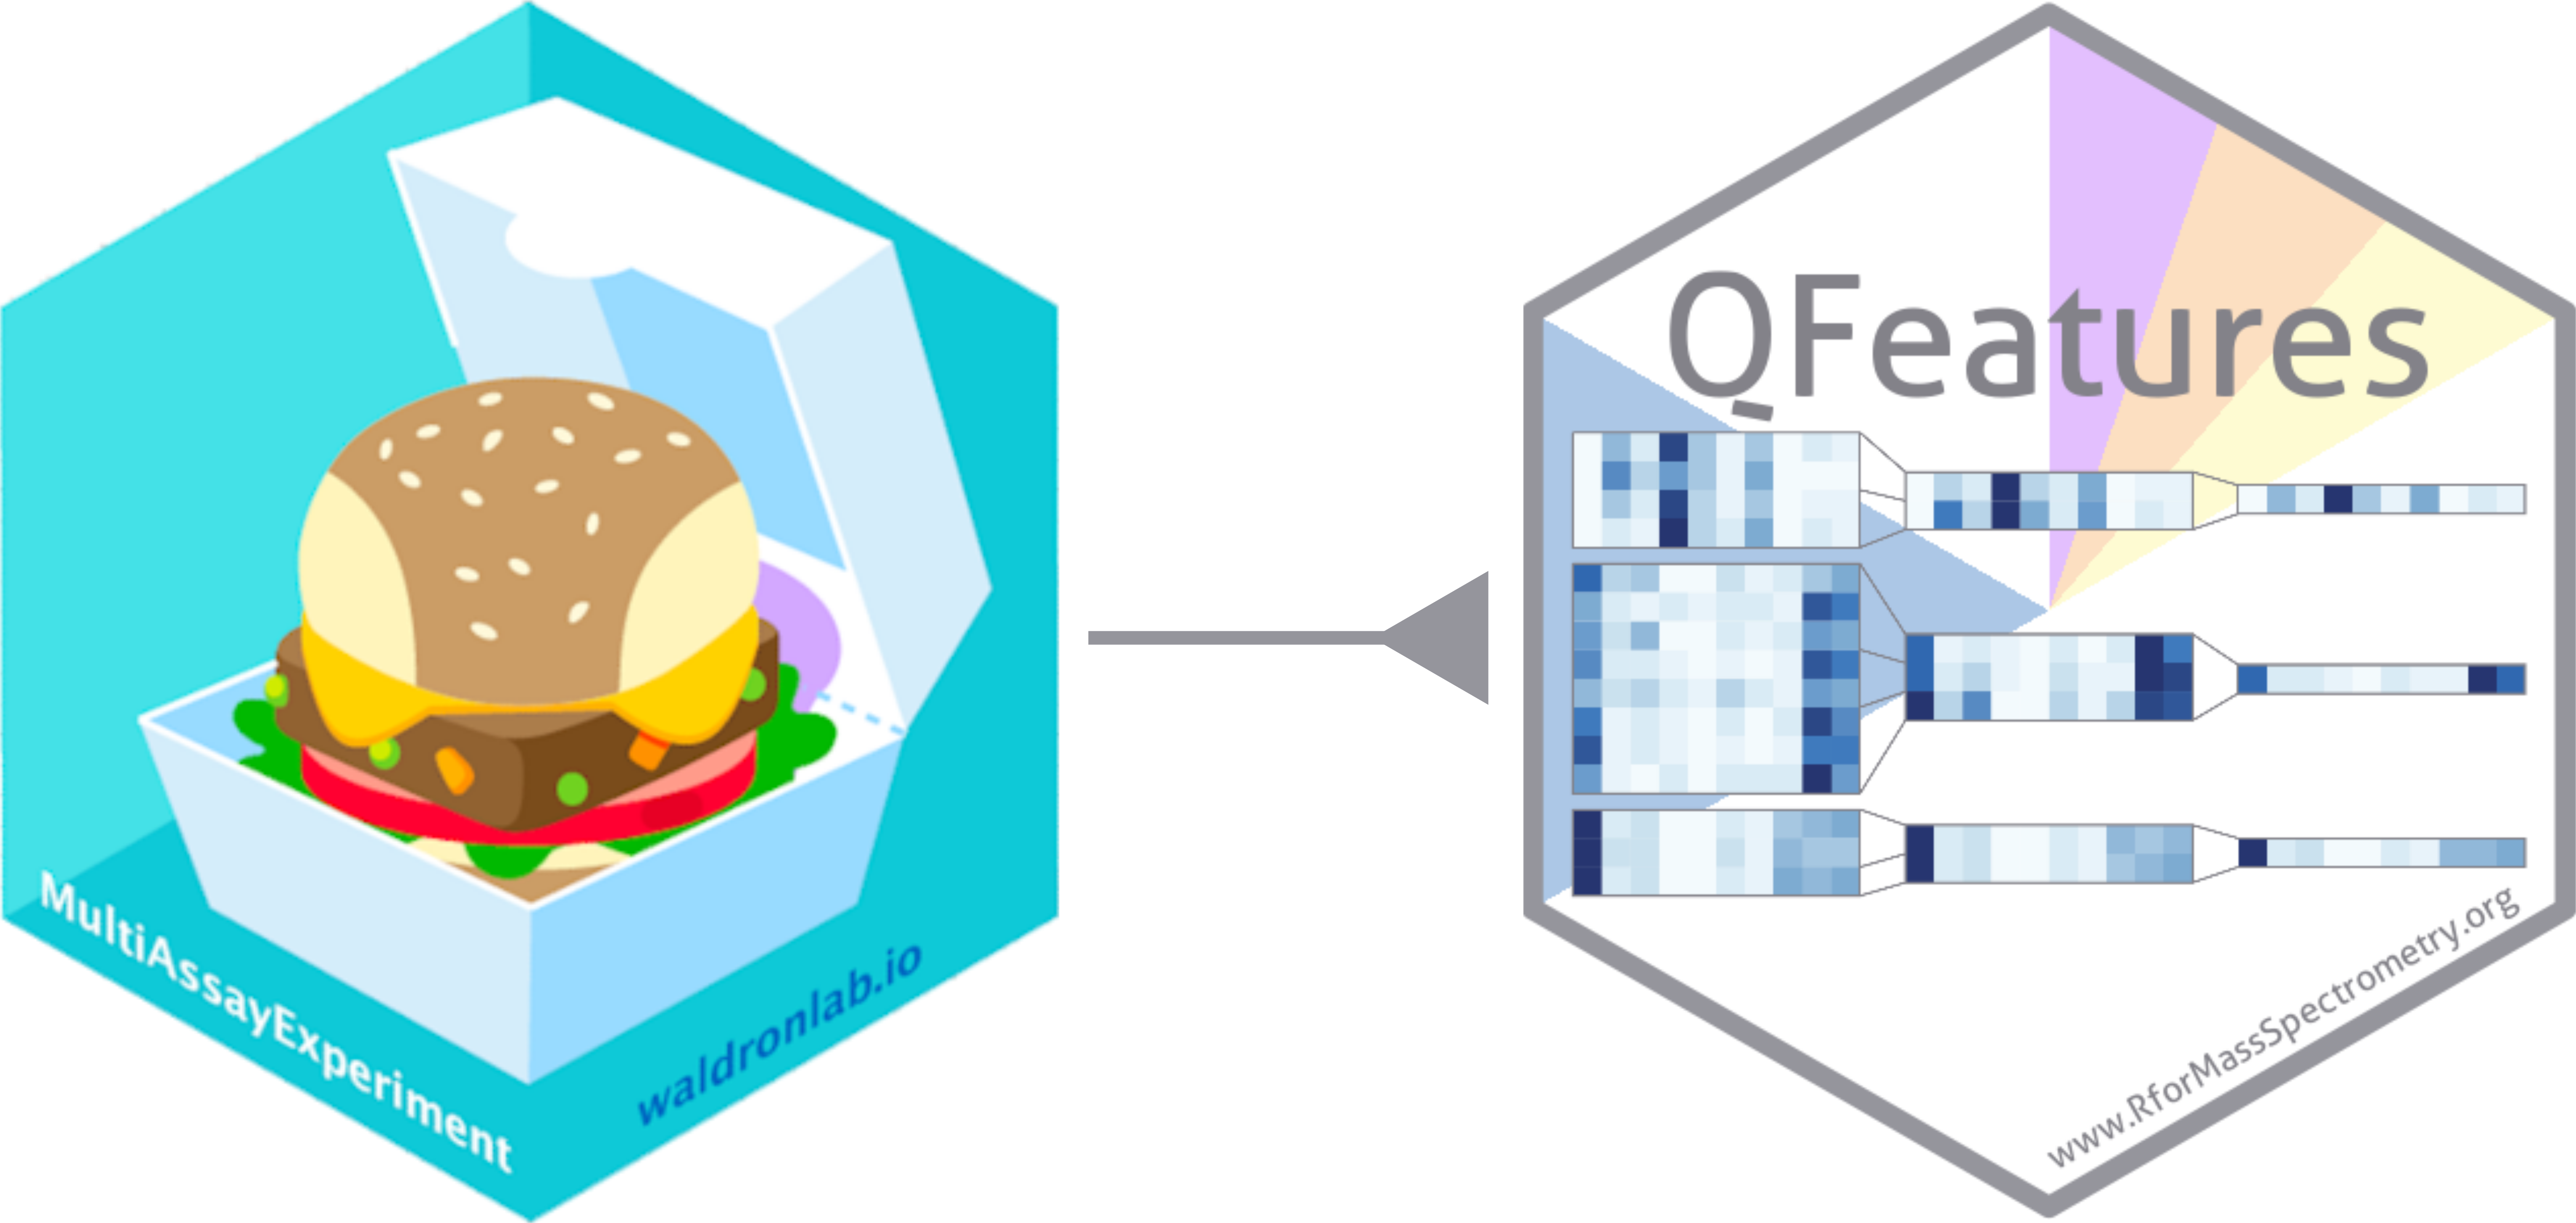
\includegraphics[width=0.7\linewidth]{figs/sticker_MAE+QFeatures.png}
  \end{columns}
  \vfill
  \begin{columns}
    \column{0.5\linewidth}
    \centering
    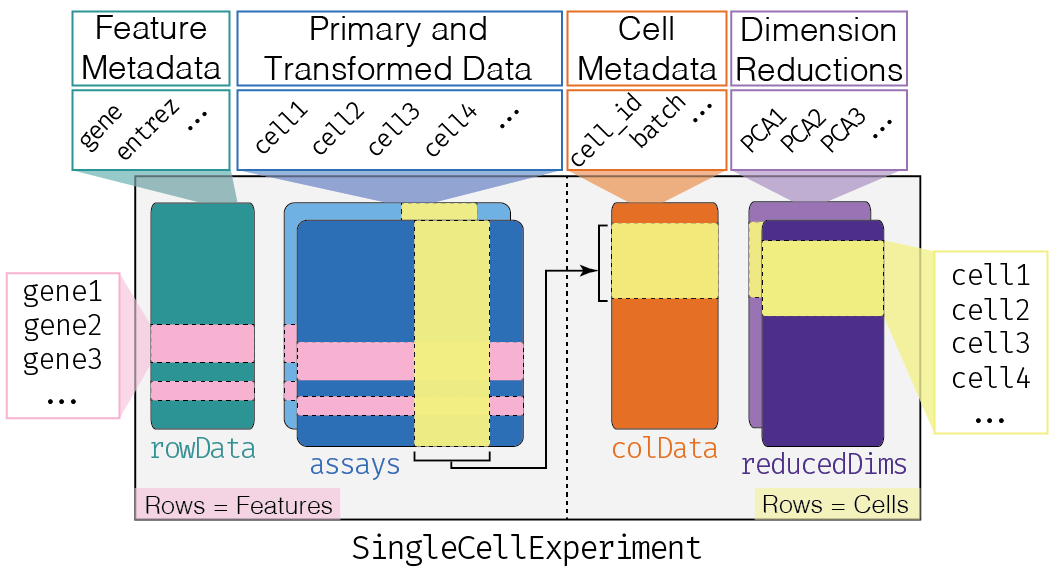
\includegraphics[width=\linewidth]{figs/SingleCellExperiment.png}
    \column{0.5\linewidth}
    \centering
    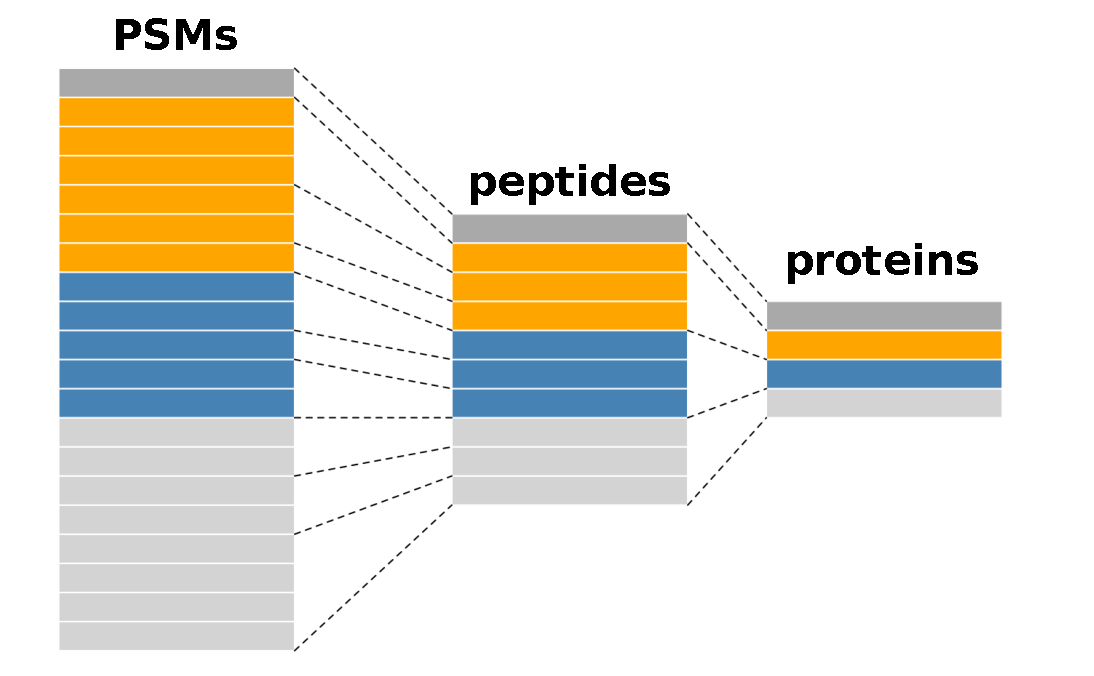
\includegraphics[width=\linewidth]{figs/QFeatures.pdf}
  \end{columns}
  
  \framebreak

  \centering
  \vfill 
  SCP data framework
  \vfill
  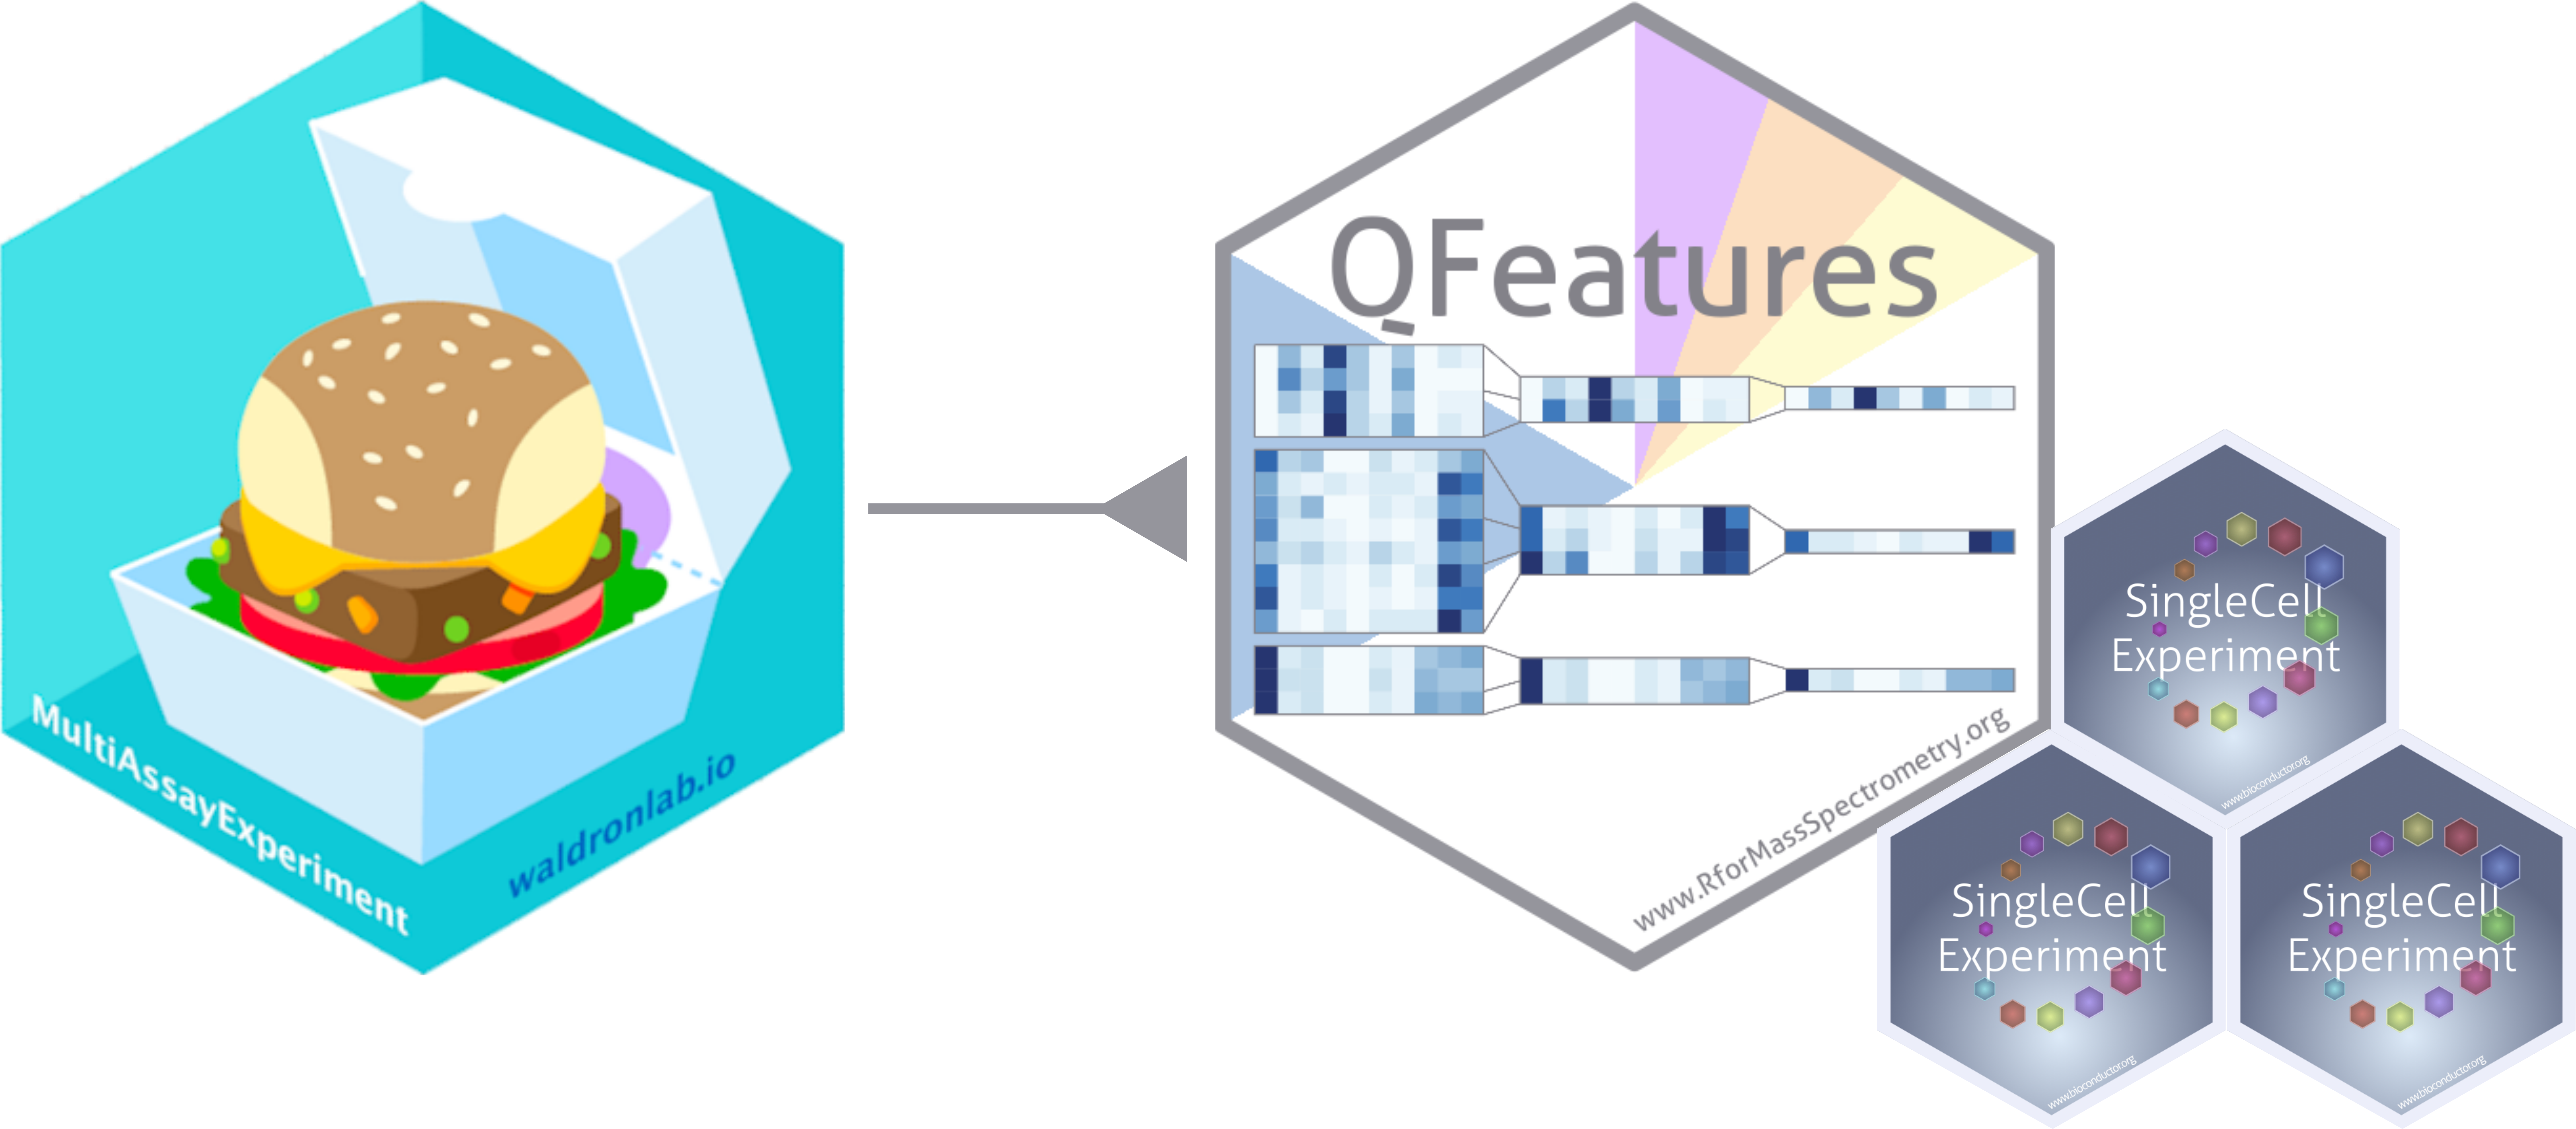
\includegraphics[width=0.4\linewidth]{figs/sticker_scp.png}
  \vfill
  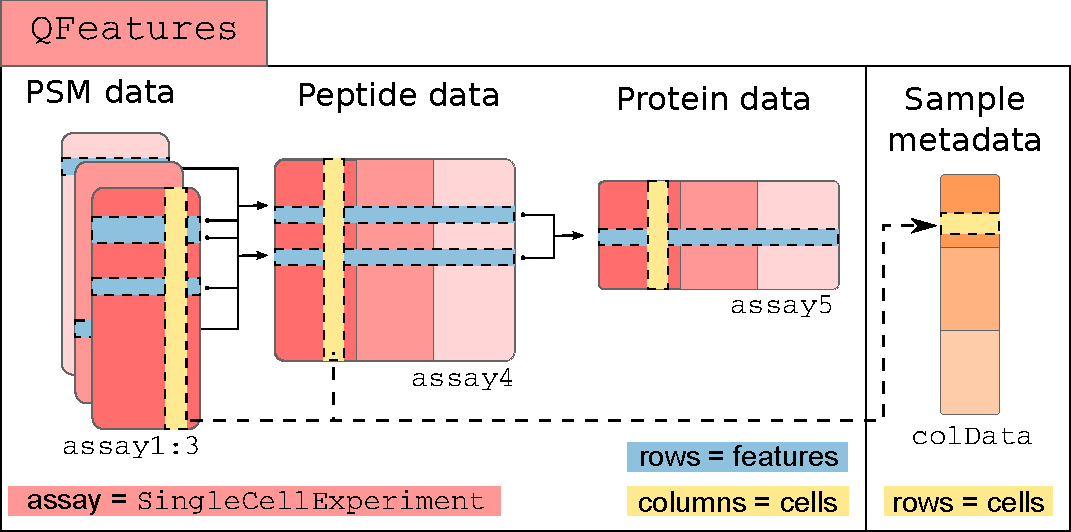
\includegraphics[width=0.9\linewidth]{figs/SCP_framework.pdf}
  
\end{frame}

%% scpdata
\begin{frame}[fragile]
  \frametitle{\hcode{scpdata}}

  \begin{columns}
    \column{0.85\linewidth}
    The package currently contains 11 datasets accessible through 
    \hcode{ExperimentHub}
    \column{0.15\linewidth}
    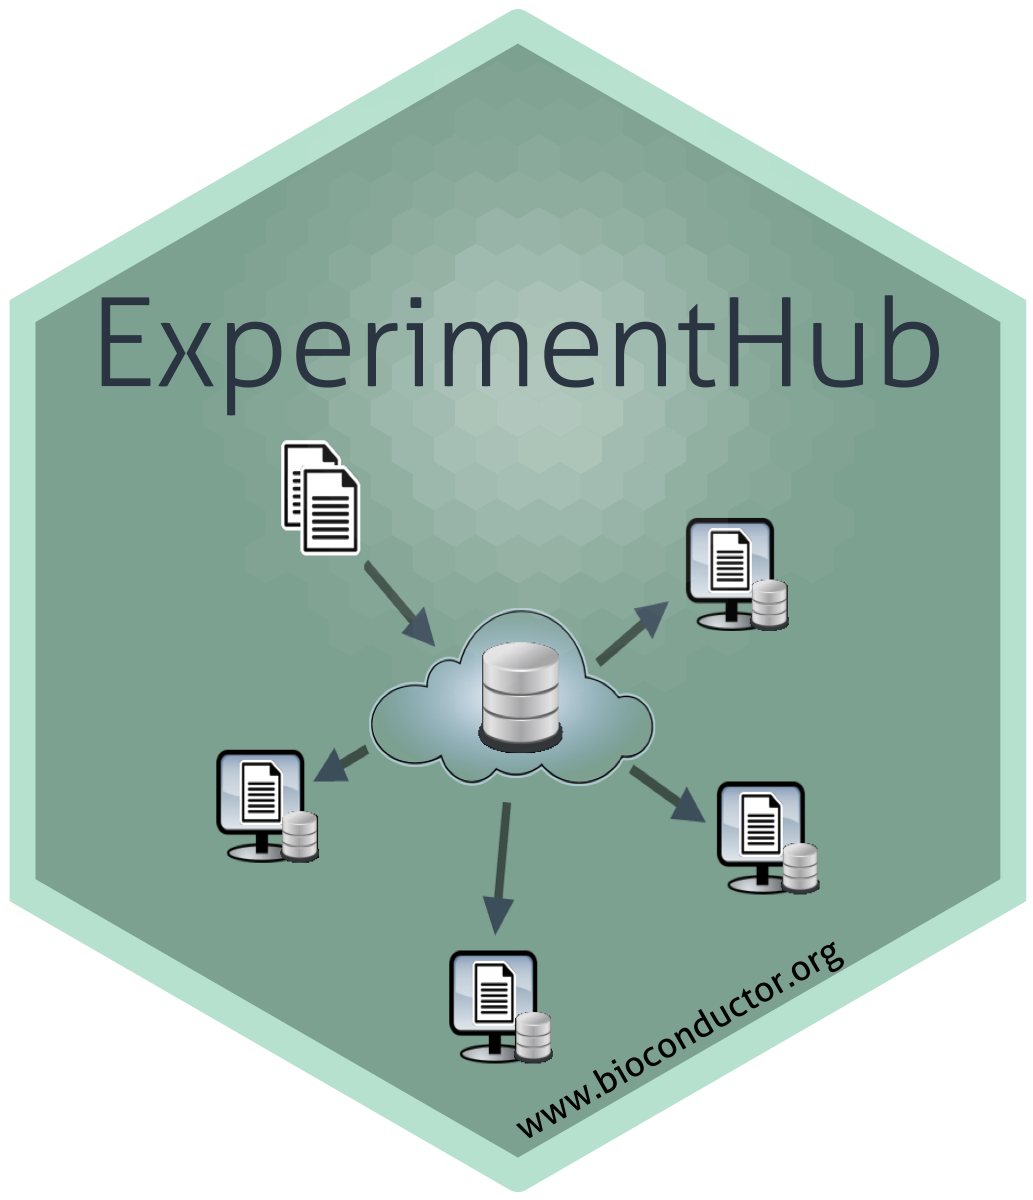
\includegraphics[width=\linewidth]{figs/sticker_EH.png}
  \end{columns}
  
  \vfill
  Example: the SCoPE2 dataset
  
  \vfill
  \begin{lstlisting}
library(scpdata)
scpd <- specht2019v3()
  \end{lstlisting}
  
  \vfill
  Overview of the dataset:
  
  \begin{lstlisting}[language={}]
show(scpd)
An instance of class QFeatures containing 179 assays:
 [1] 190222S_LCA9_X_FP94AA: SingleCellExperiment with 2823 rows and 11 columns 
 [2] 190222S_LCA9_X_FP94AB: SingleCellExperiment with 4297 rows and 11 columns 
 [3] 190222S_LCA9_X_FP94AC: SingleCellExperiment with 4956 rows and 11 columns 
 ...
 [177] 191110S_LCB7_X_APNOV16plex2_Set_9: SingleCellExperiment with 4626 rows and 16 columns 
 [178] peptides: SingleCellExperiment with 9208 rows and 1018 columns 
 [179] proteins: SingleCellExperiment with 2772 rows and 1018 columns 
  \end{lstlisting}
  
\end{frame}
 
%% scp
\begin{frame}[fragile]
  \frametitle{\hcode{scp}}
 
  \begin{columns}
    \column{0.3\linewidth}
    \footnotesize
    SCoPE2 pipeline:\\
    \begin{enumerate}
      \item Input data
      \item QC on features
      \item Peptide aggregation
      \item QC on samples
      \item Log-normalization
      \item Feature selection
      \item Protein aggregation 
      \item Imputation
    \end{enumerate}
    
    \column{0.8\linewidth}
    
    \begin{lstlisting}
readSCP(quantTable = quantData, 
        metaTable = metaData,
        channelCol = "Channel", 
        batchCol = "Set") %>%
  zeroIsNA(i = 1:4) %>%
  computeSCR(i = 1:4, 
             colDataCol = "SampleType",
             carrierPattern = "Carrier",
             samplePattern = "Monocyte") %>%
  filterFeatures(~ Potential.contaminant != "+" & 
                   .meanSCR < 0.1) %>%
  subsetByAssay(dims(.)[1, ] > 150) %>%
  joinAssays(i = 4:6, name = "peptides") %>%
  computeMedianCV(i = 1:3, 
                  proteinCol = "protein",
                  peptideCol = "peptide") %>%
  subsetByColumn(.$MedianCV < 0.4) %>%
  normalize(i = "peptides", 
            method = "median", na.rm = TRUE) %>%
  logTransform(i = "normAssay",
               base = 2) %>%
  aggregateFeatures(i = "logAssay", 
                    name = "proteins",
                    fcol = "protein") %>%
  impute(i = "normAssay",
         method = "knn") ->
  scp
    \end{lstlisting}
  \end{columns}
\end{frame}



%% SCoPE2 replication results
\begin{frame}
  \frametitle{SCoPE2 replication results}
  
  \vfill
  \begin{columns}
  
    \column{0.33\linewidth}
    Cell filter\\
    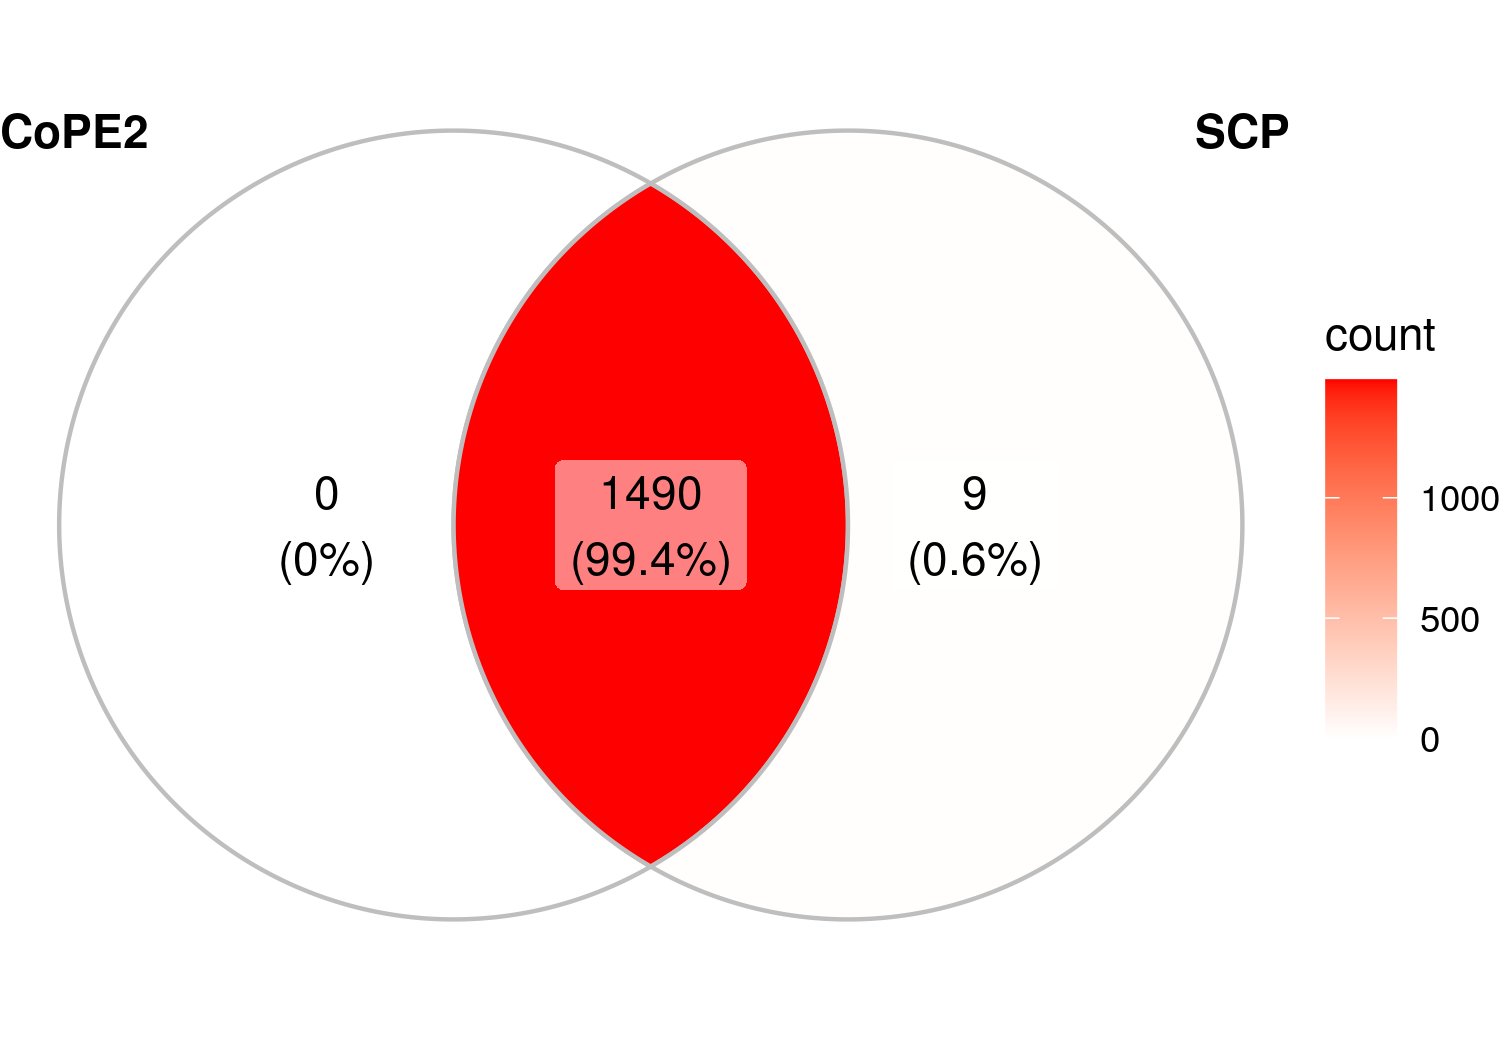
\includegraphics[width=\linewidth]{figs/cell_filter.png}\\
    Protein filter\\
    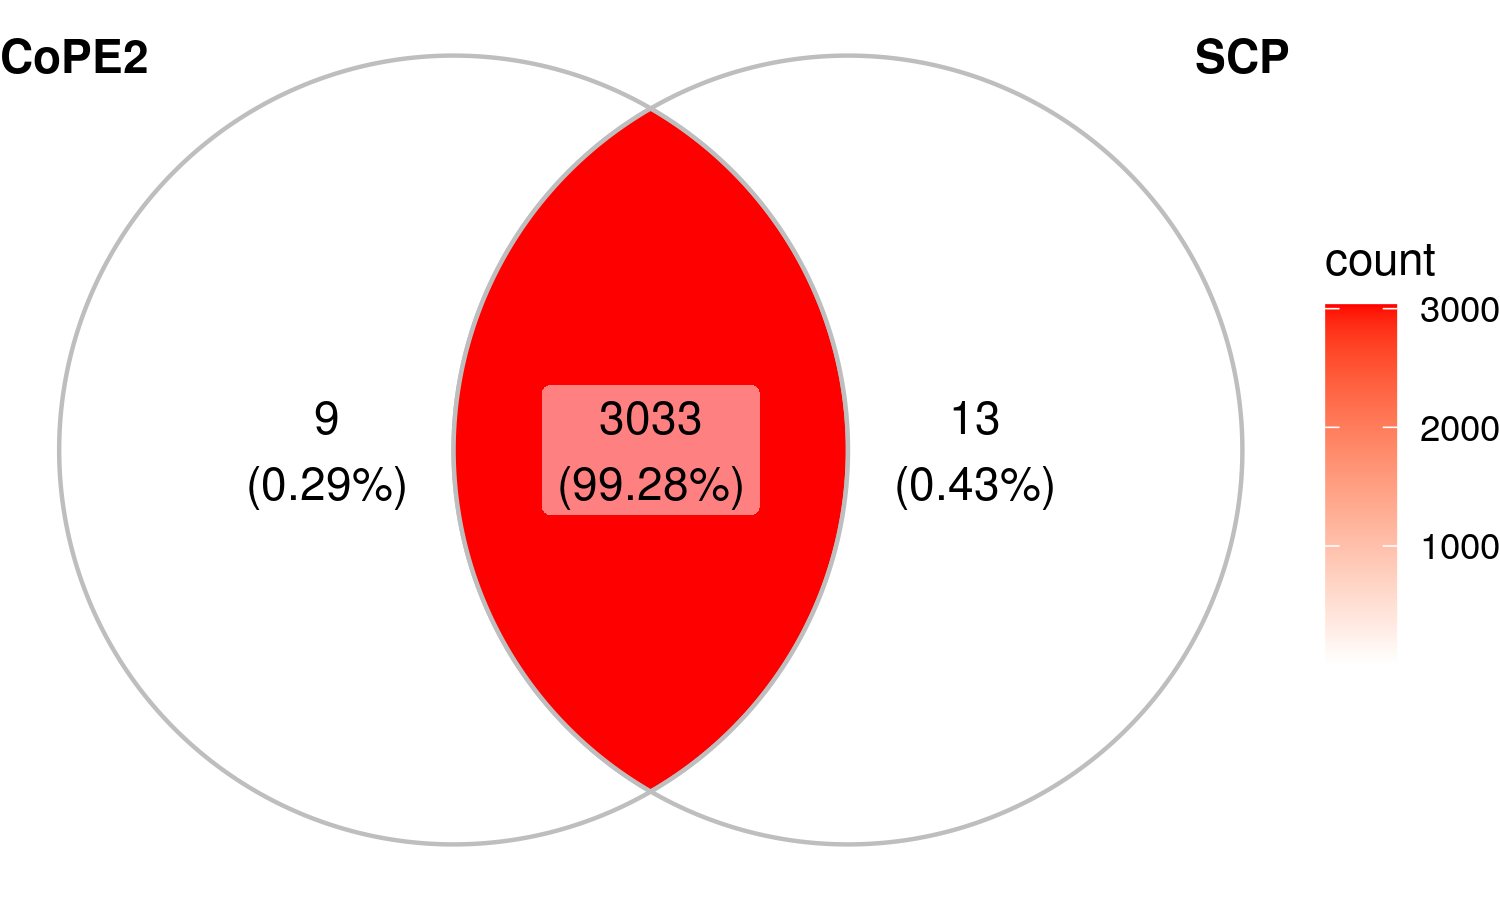
\includegraphics[width=\linewidth]{figs/protein_filter.png}\\
  
    \column{0.33\linewidth}
    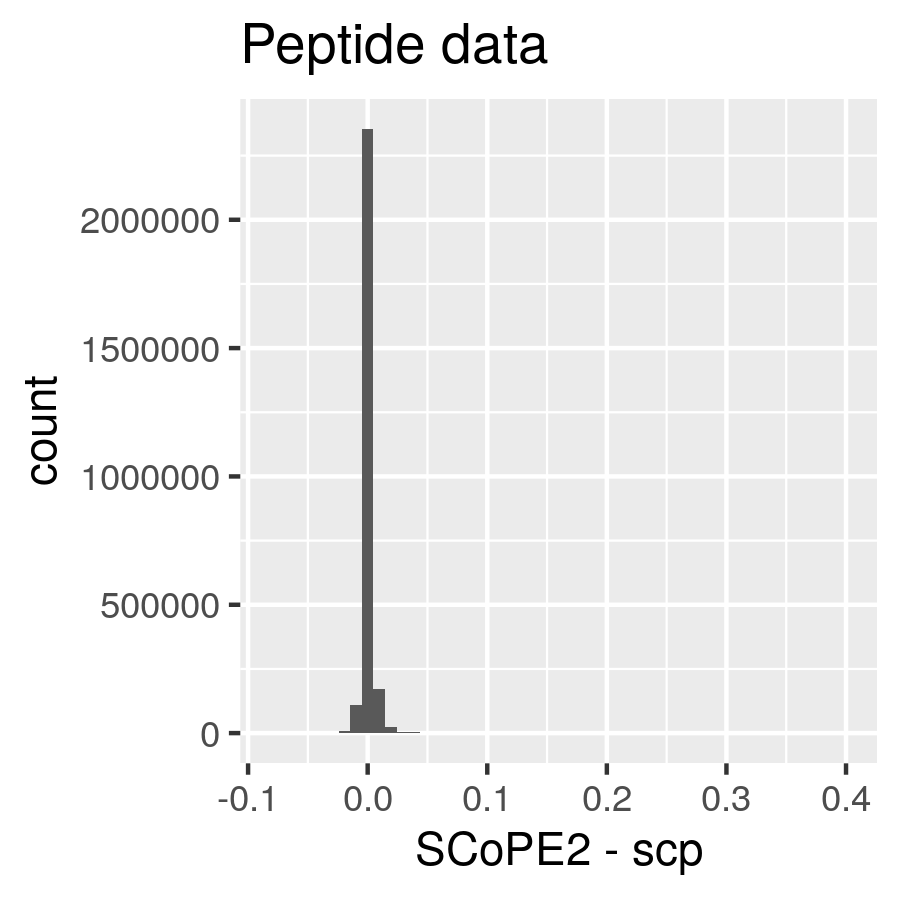
\includegraphics[width=\linewidth]{figs/peptide_error.png}
  
    \column{0.33\linewidth}
    SCoPE2\\
    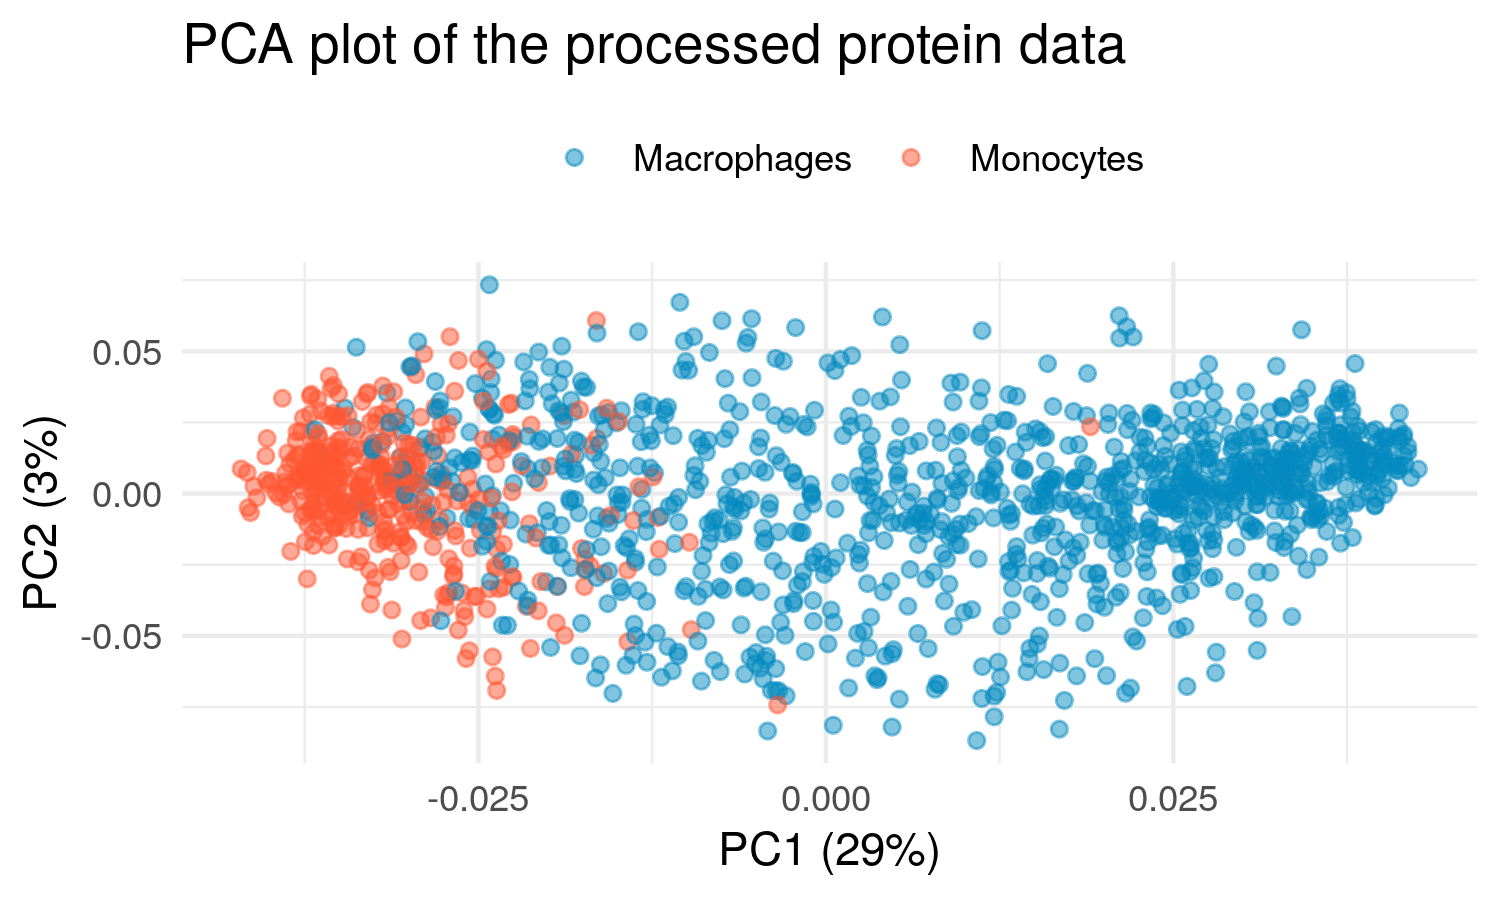
\includegraphics[width=\linewidth]{figs/wPCA_SCoPE2.png}
    \hcode{scp}\\
    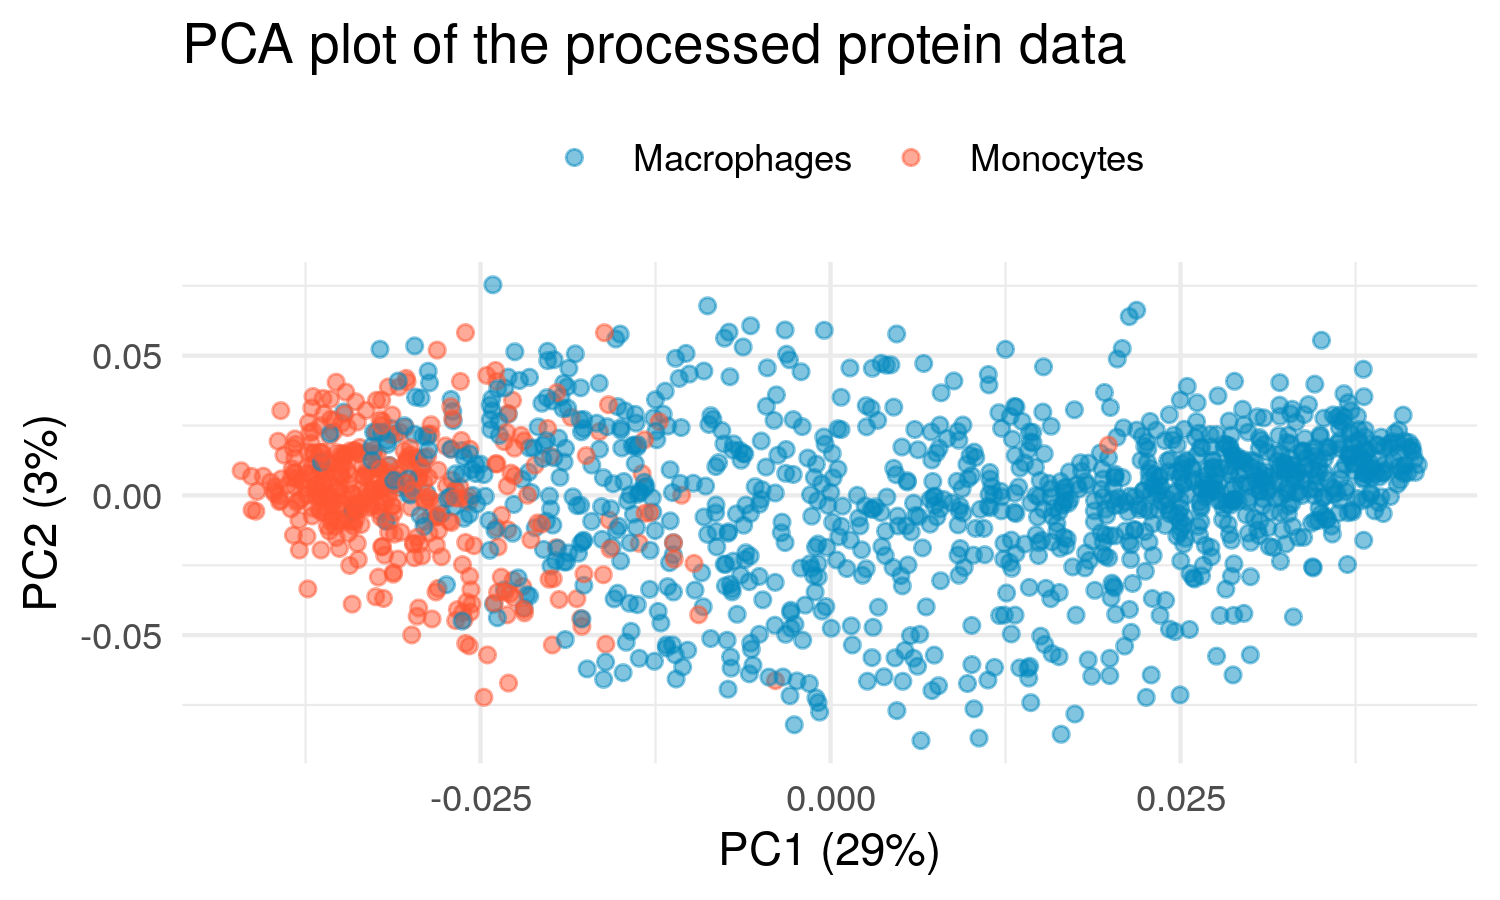
\includegraphics[width=\linewidth]{figs/wPCA_scp.png}
  
  \end{columns}
  
\end{frame}

%% Replication progress
\begin{frame}
  \frametitle{Replication progress}
  
  We used \hcode{scp} to reproduce 2 SCP analyses:
  
  \vfill
  \begin{enumerate}
    \item Successful replication of SCoPE2 analysis (multiplexed) + 
    identification of \textbf{issues and improvements} to the analysis
    \item Failed replication of \cite{Zhu2019-ja} (label-free): lack 
    of good documentation
  \end{enumerate}
  
  \vfill
  This demonstrate the successful application of our software to 
  various SCP datasets. 
  
  \vfill
  \begin{columns}
    \column{0.1\linewidth}
    \raggedleft
    
\includegraphics[width=\linewidth]{figs/under_construction.png}
    \column{0.9\linewidth}
    Preprint is being written
  \end{columns}
  
\end{frame}

%% Single-cell challenges
\begin{frame}[c]
  \frametitle{Single-cell challenges}
  
  \begin{center}
    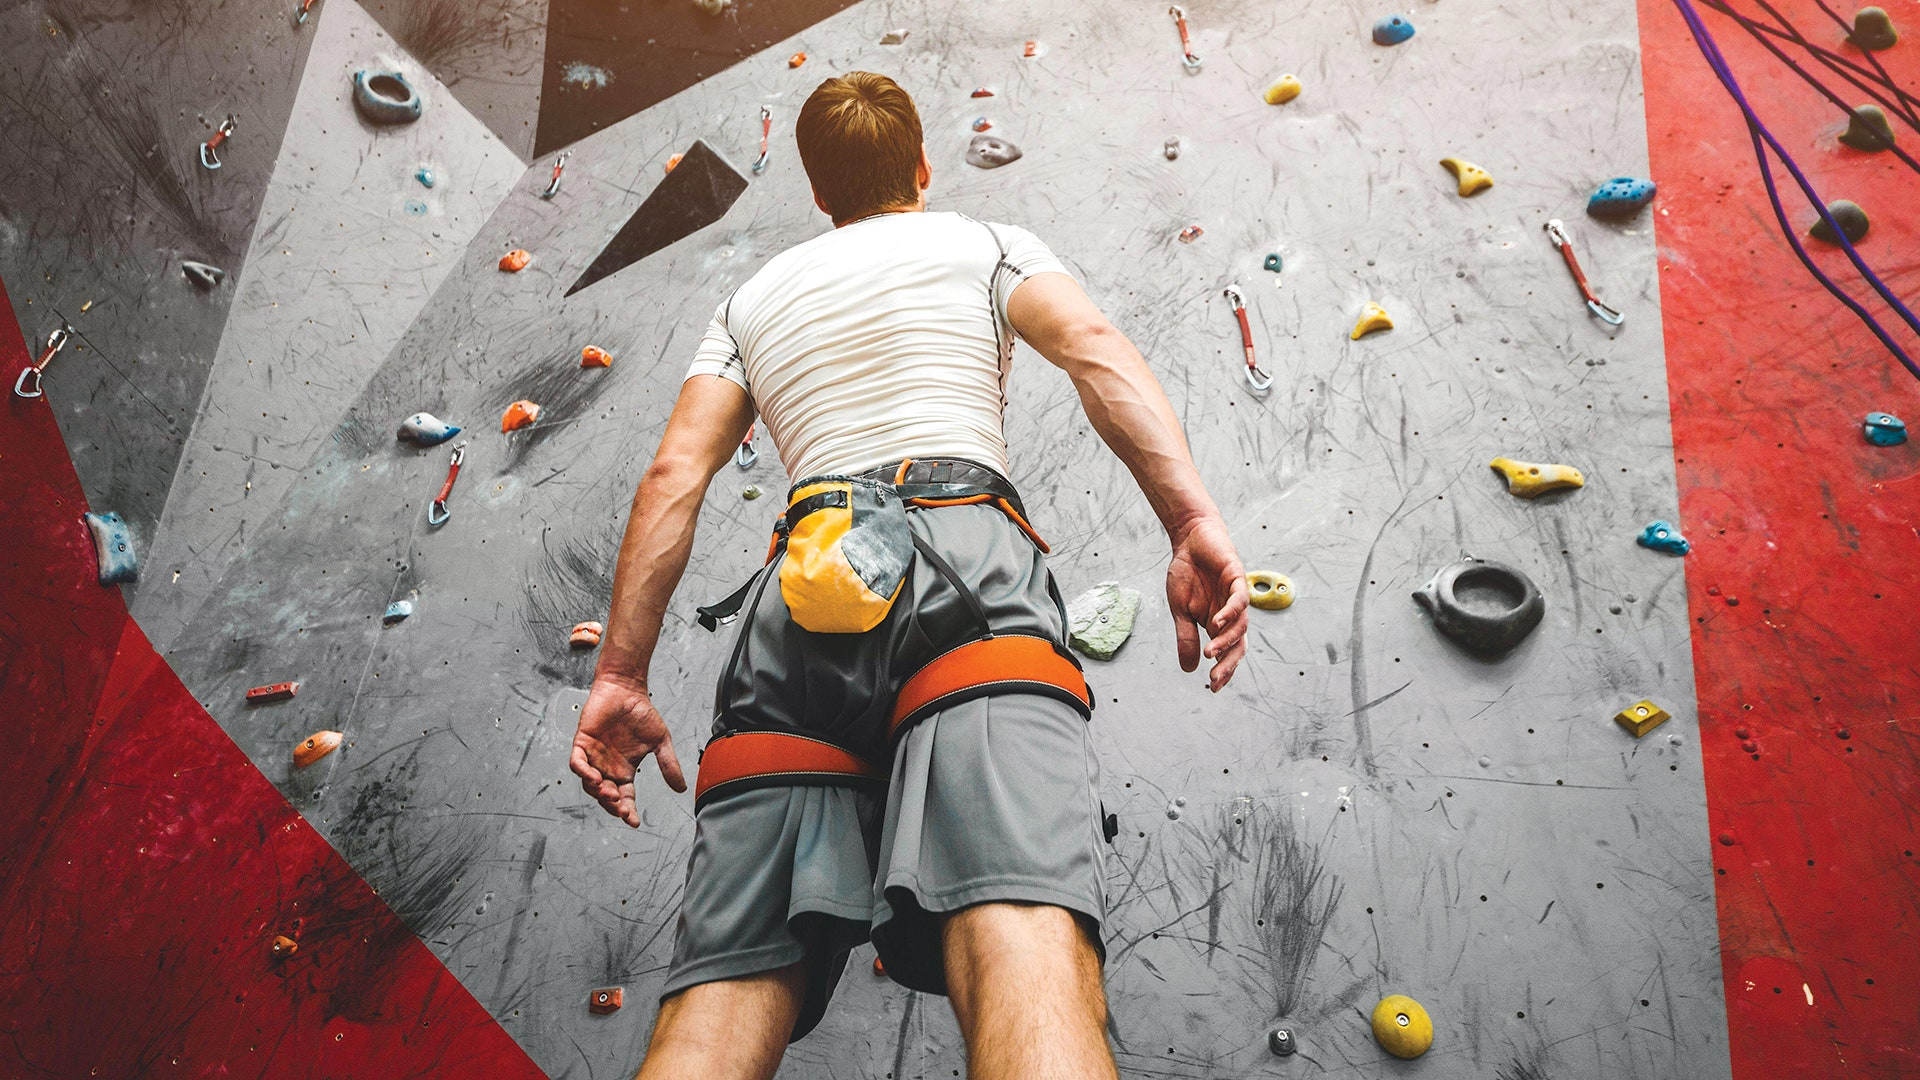
\includegraphics[width=0.5\linewidth]{figs/climb.jpg}
  \end{center}
  
  \pause
  
  \vfill
  \begin{itemize}
    \item Technical challenges: automation, minute sample amount, cost 
      per cell
    \item Computational challenges: big data, missingness, complex
      batch effects
    \item Conceptual challenges: what is a cell type? what is 
      biologically relevant? 
  \end{itemize}
  
  
\end{frame}
    
%% SCP challenges: batch effect
\begin{frame}
  \frametitle{SCP challenges: batch effect}
  
  \begin{columns}
    \column{0.6\linewidth}
    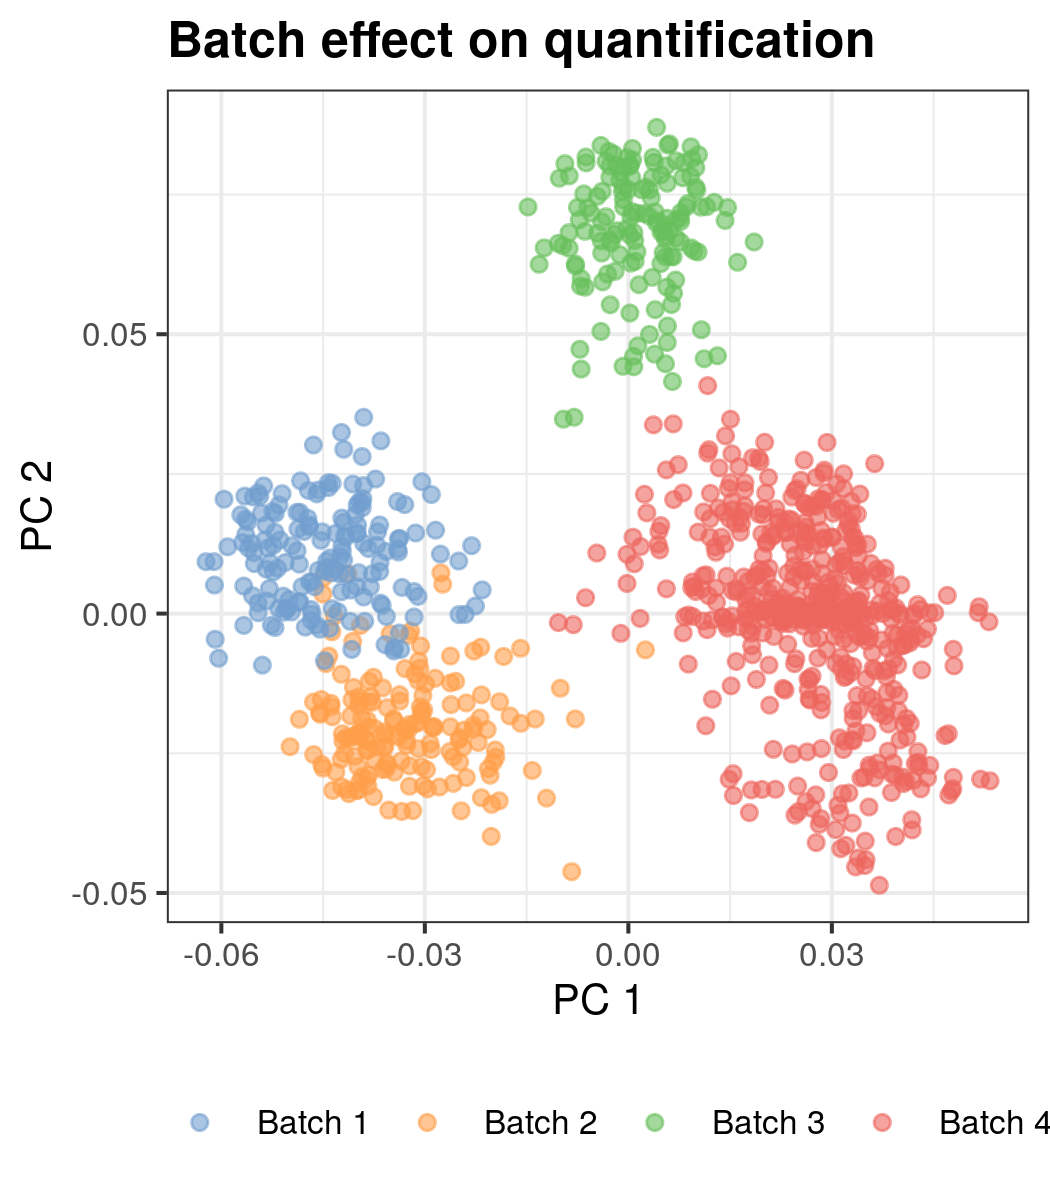
\includegraphics[width=\linewidth]{figs/PCA_batch_effect.png}
    \column{0.4\linewidth}
    \begin{itemize}
      \item Sample collection batch
      \item Chromatographic batch
      \item Mass spectrometer maintenance
    \end{itemize}
    SCoPE2 analysis removed batch effects using \hcode{ComBat}
  \end{columns}
  
\end{frame}

%% SCP challenges: missingness
\begin{frame}
  \frametitle{SCP challenges: missingness}
  
  \centering
  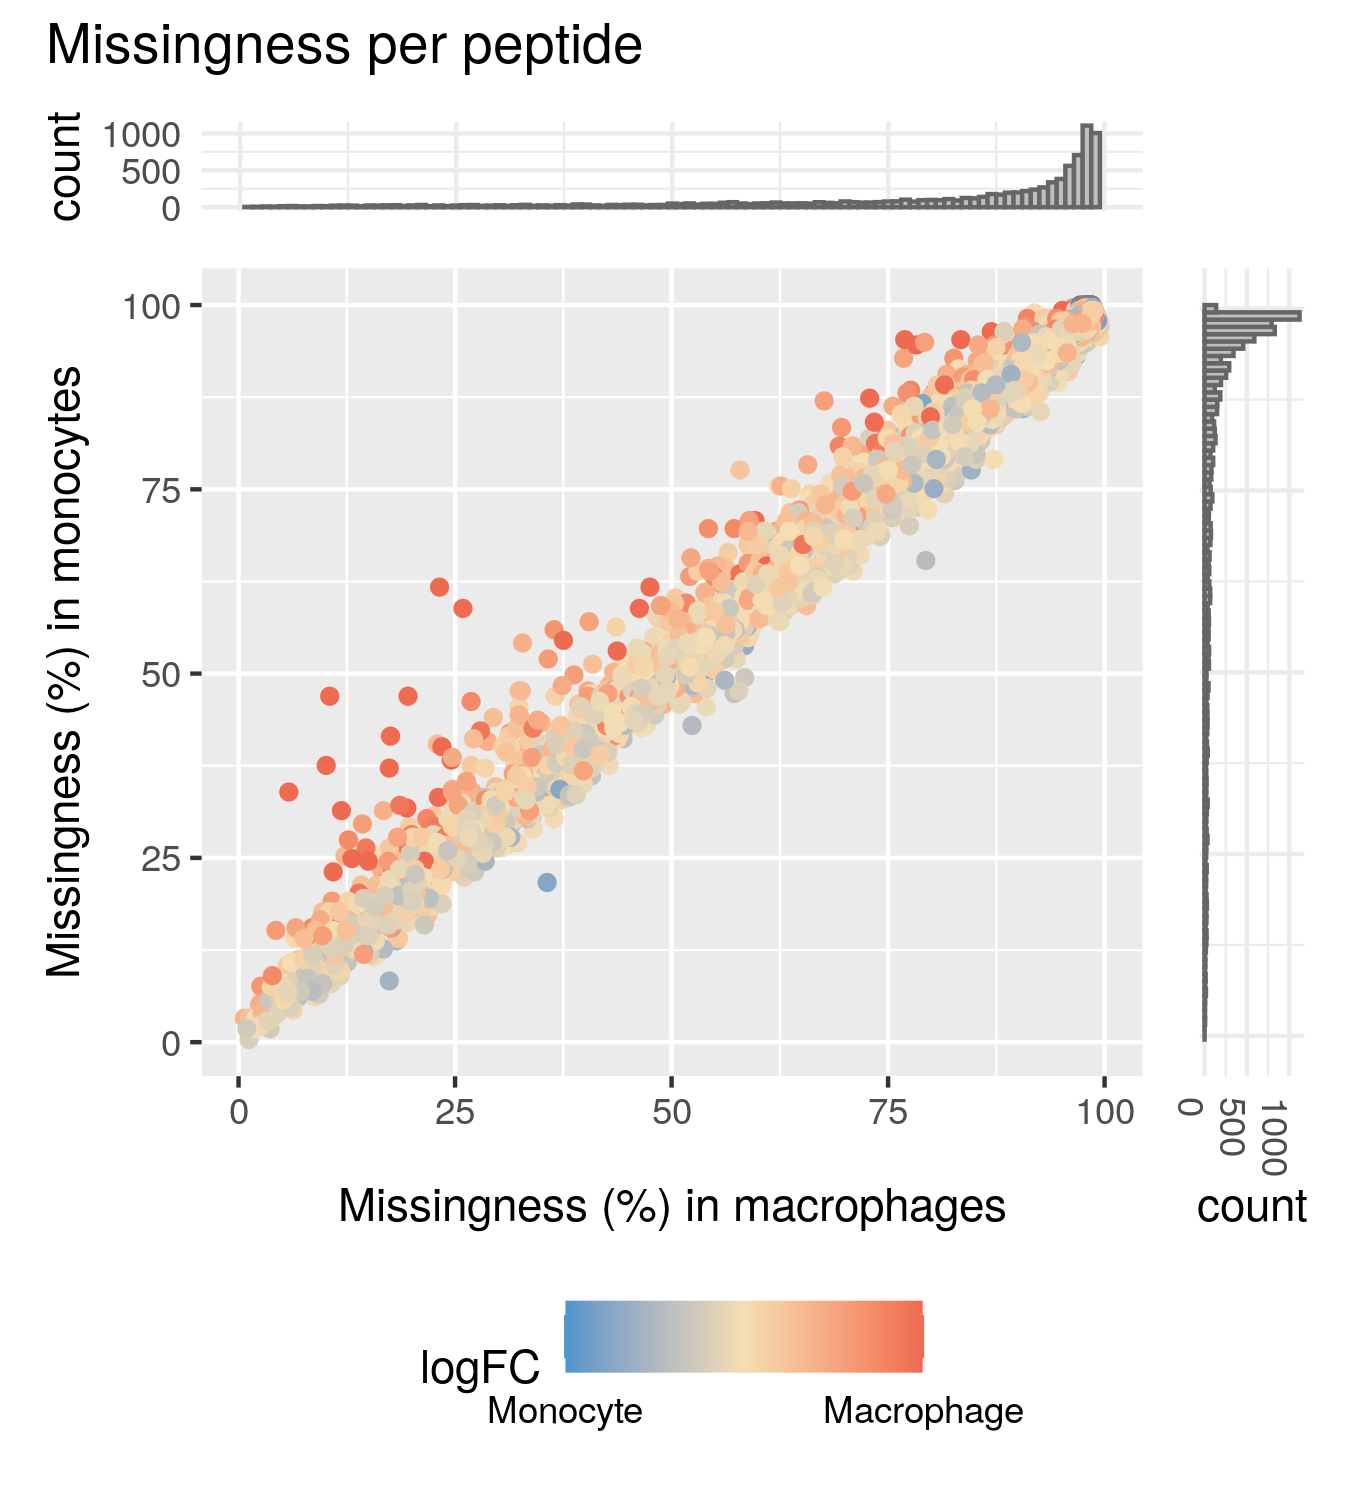
\includegraphics[width=0.6\linewidth]{figs/missing_peptide.png}
  
\end{frame}


%% SCP challenges: batch effect + missingness
\begin{frame}
  \frametitle{SCP challenges: batch effect + missingness}
  
  \centering
  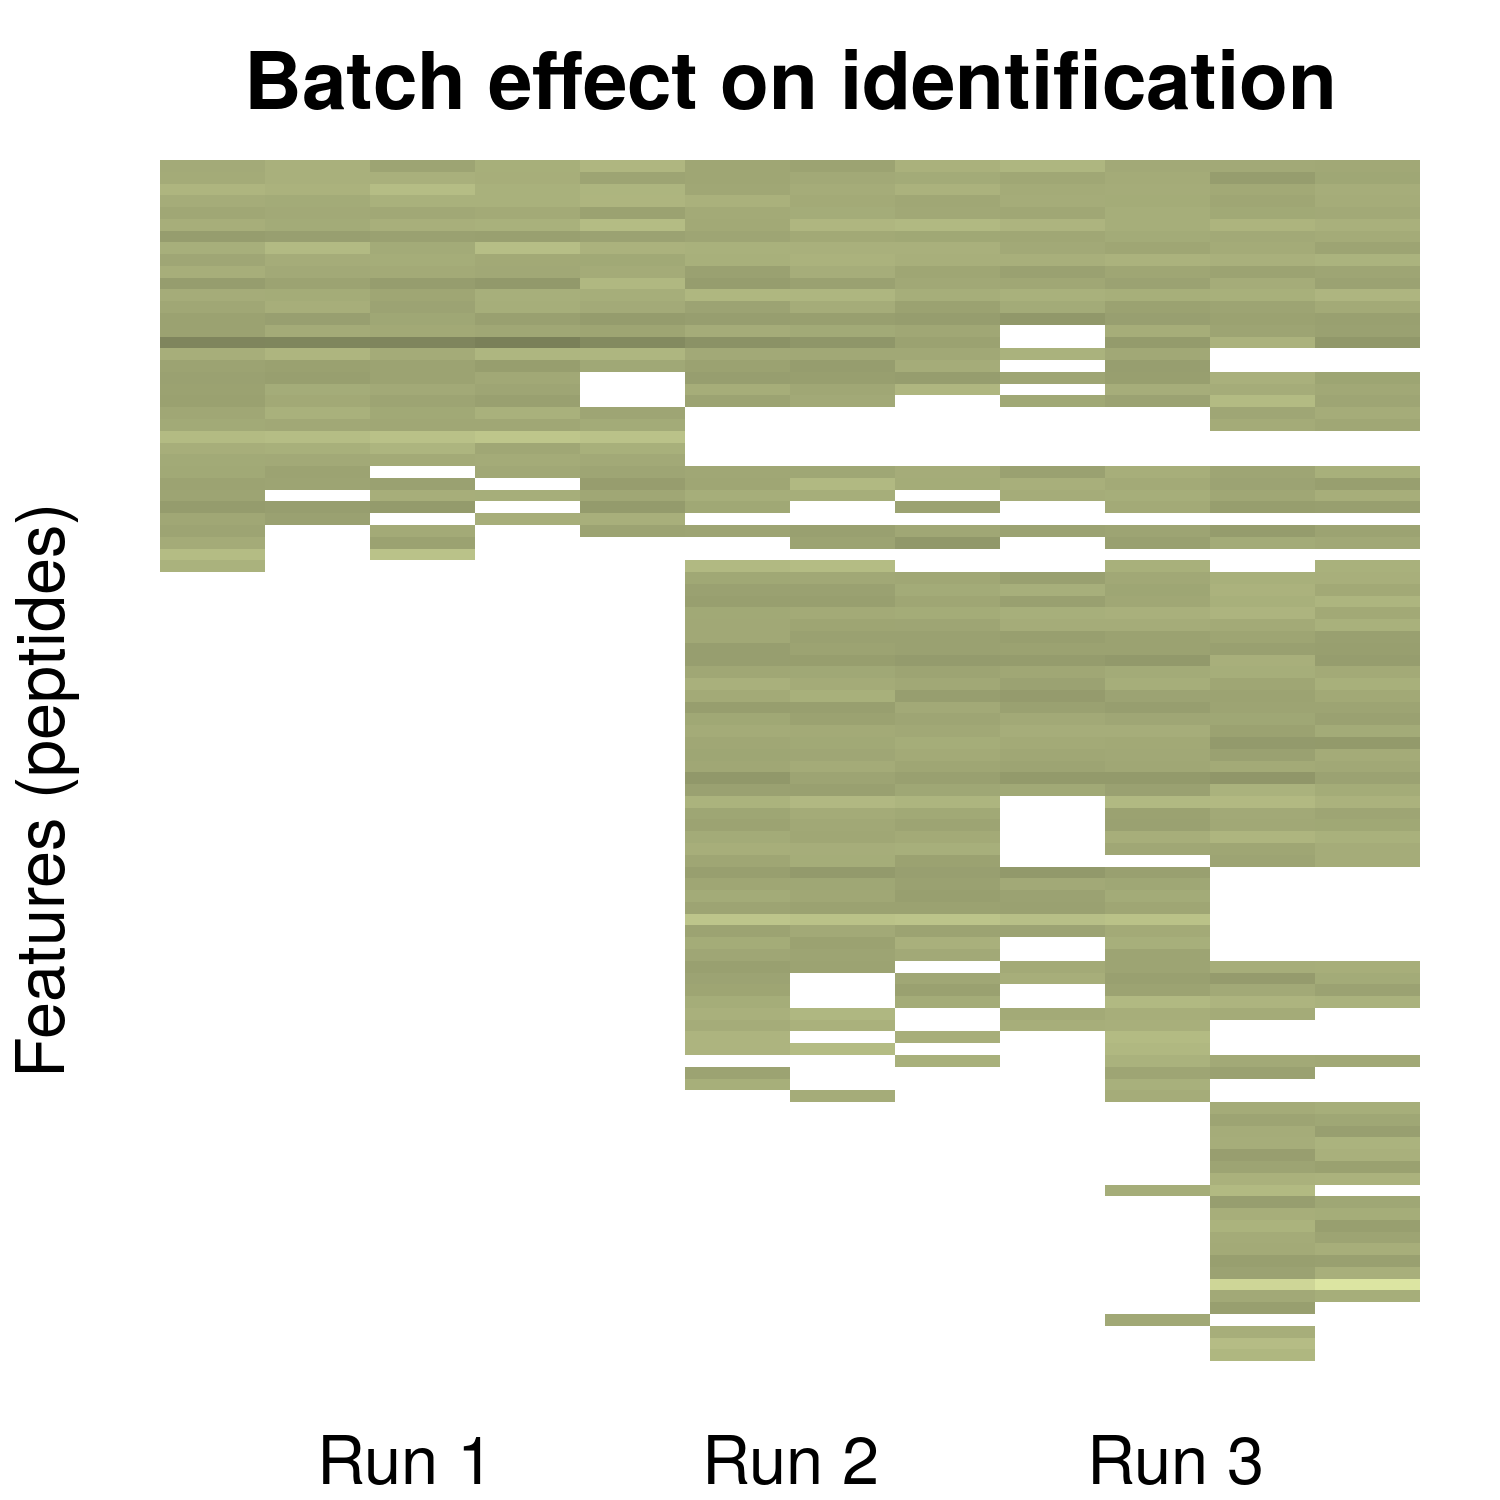
\includegraphics[width=0.6\linewidth]{figs/batch_effects.png}

\end{frame}

%% Takehome message
\begin{frame}
  \frametitle{Takehome message}
  
  \begin{itemize}
    \item SCP is an emerging but very promising field!
    \item We developed a computational infrastructure to formalize SCP
      data analyses
    \item The infrastructure could be applied to reproduce 2 published 
      analyses
    \item Exciting challenges are yet to be solved
  \end{itemize}
  
  \vfill
  \includegraphics[width=\linewidth]{figs/conclusion.pdf}
  
\end{frame}

%% Acknowledgements
\begin{frame}[b]
  \frametitle{Acknowledgements}
  \centering
  
  \begin{itemize}
    \item UCLouvain-CBIO lab: Laurent Gatto
    \item Slavov lab: Nikolai Slavov,  Harrison Specht
    \item Bioconductor team: Lori Shepherd
    \item Bioconductor and EuroBioc community
    
  \end{itemize}
  
  \vfill
  Thank you for your attention!

  \footnotesize 
  I'm happy to take questions now or at the discussion tables
  
  \vfill
  \begin{columns}
    \column{0.4\linewidth}
    
\includegraphics[width=\linewidth]{figs/ucl.png}
    \column{0.4\linewidth}
    \column{0.2\linewidth}
    
\includegraphics[width=\linewidth]{figs/fnrs.png}
  \end{columns}
\end{frame}



%-----------------------------------------------
% References
%-----------------------------------------------

\begin{frame}[allowframebreaks]{References}
  \scriptsize
  \bibliographystyle{plainnat}
  \bibliography{ref}
\end{frame}


\end{document}
